\documentclass[11pt]{article}
\usepackage{fullpage}
\usepackage[left=1.27cm,top=1.25cm,right=1.27cm,bottom=1.25cm,headheight=2ex,headsep=3ex]{geometry}
\usepackage{graphicx}
\usepackage{float}
\usepackage{graphicx}
\usepackage[table,xcdraw]{xcolor}
\usepackage{enumerate}
\usepackage{colortbl}
\usepackage{hyperref}
% Idioma
\usepackage[spanish,es-tabla]{babel}
\selectlanguage{spanish}
\decimalpoint
\usepackage[utf8]{inputenc}
% Para pies de tabla y de figura
\usepackage{caption}
% tcolorbox 
\usepackage[most]{tcolorbox}
\usepackage{tikz}
% Color definitions
\definecolor{raspberry}{rgb}{0.89, 0.04, 0.36}
\definecolor{yelltcol}{HTML}{FEE581}
% Tablas con line break automático
\usepackage{tabularx}
% Colores para tabla

\definecolor{bluerow}{HTML}{D5E5FF}
\definecolor{redrow}{HTML}{FFAAAA}
\definecolor{purplerow}{HTML}{FFAAEE}

\newtcolorbox{mybox}[2][]{%
	enhanced,
	colbacktitle=red!10!white,
	colback=blue!10!white,
	coltitle=raspberry!90!black,
	attach boxed title to top left={xshift=1cm,yshift=-\tcboxedtitleheight/2,yshifttext=-\tcboxedtitleheight/2},
	%attach boxed title to top center={yshift=-2mm},
	title={#2},
	drop fuzzy shadow southeast,%=black!50!white,
	fonttitle=\bfseries,
	#1
}
\usepackage{fontawesome}
%\usepackage{enumitem}

\newenvironment{tight_enumerate}{
	\begin{enumerate}
		\setlength{\itemsep}{0pt}
		\setlength{\parskip}{0pt}
	}{\end{enumerate}}

\title{
\includegraphics[width=0.2\textwidth]{logo_ITESO.png}\\%
		Departamento de Matemáticas y Física\\
		GUÍA DE APRENDIZAJE \\
		{\bf Decisiones y Teoría de Juegos}}
\author{%
  % The Author 
}
\date{}

\begin{document}

\maketitle
\vspace*{-2em}
\begin{table}[ht]
	\centering
	\begin{tabular}{|>{\columncolor[gray]{0.9}}l|l|l|l|l|l|}
		\hline
		Asignatura:      & \multicolumn{3}{l|}{DECISIONES   Y TEORÍA DE JUEGOS}          & \cellcolor[gray]{0.9} Créditos   BCD:       &        4       \\ \hline
		Clave:           &      MAF1301ITE2134                                     & \cellcolor[gray]{0.9} Grupo:  &         & \cellcolor[gray]{0.9} Créditos   TIE:       &        4       \\ \hline
		Carreras         & Ingeniería Financiera                     & \cellcolor[gray]{0.9} Horario: &  18:00-20:00  & \cellcolor[gray]{0.9} Aula: (L, Mi)   & D-203; J-SDEMO         \\ \hline
		Departamento:    & \vtop{\hbox{\strut Departamento de} 
						   \hbox{\strut Matemáticas y Física}}       & \cellcolor[gray]{0.9} UAB:    &         & \cellcolor[gray]{0.9} Periodo:              & Primavera 2022 \\ \hline
		Coordinador UAB: & \multicolumn{2}{l|}{Juan Diego Sánchez Torres}       & \cellcolor[gray]{0.9} E-mail: & dsanchez@iteso.mx     & Ext 3069       \\ \hline
		Profesor:        & \multicolumn{2}{l|}{Emmanuel Alcalá Temores}   & \cellcolor[gray]{0.9} E-mail: & jaime.alcala@iteso.mx &                \\ 
		\hline
	\end{tabular}
\end{table}



\section{Presentación}

La Teoría de juegos es un área de las matemáticas aplicadas que hace uso de herramientas formales, como la teoría de la probabilidad, teoría de grafos y cálculo para resolver problemas de decisión que involucran a múltiples agentes, cuyas ganancias son interdependientes.
% La teoría de juegos es una poderosa herramienta que hace uso de la matemática, la probabilidad y el análisis para resolver problemas en los que están involucradas decisiones en las que participa más de un agente. En la economía financiera se utiliza principalmente en modelos de comportamiento de las empresas en los mercados de factores, o para dilucidar problemas de decisión multiagente dentro de ellas. 

Decisiones y Teoría de Juegos se divide en cuatro unidades. En cada una de esta se presenta un tipo de juego distinto que corresponde a las distintas situaciones reales que pueden ser modeladas, y en ese sentido simplificadas, mediante las herramientas formales de la teoría. Primero, comenzamos con los fundamentos de teoría de decisión, introduciendo la teoría de elección racional; posteriormente, se presentan los juegos estáticos con información completa; en la segunda unidad, se presentan los juegos dinámicos o secuenciales con información completa. En la tercera y cuarda unidades se introducen los juego bayesianos, en donde exigimos de nuestros jugadores que se representen la incertidumbre de forma probabilística; en la tercera, se presentan los juegos estáticos con información incompleta, y finalmente los juegos dinámicos con información incompleta.

Correspondiendo a estas cuatro clases de juegos hay tres nociones de equilibrio, cada una considerada un refinamiento de su antecesora: el equilibrio de Nash, el equilibrio de Nash perfecto en subjuegos, el equilibrio bayesiano de Nash y el equilibro bayesiano perfecto.

\section{Contextualización de la asignatura}

Esta materia es impartida para estudiantes de la carrera de Ingeniería Financiera y se sugiere cursarla en el sexto semestre. Se requieren competencias y conocimientos en teoría de la probabilidad, cálculo, álgebra lineal y preferentemente conocimiento de un lenguaje de programación en el que puedan expresar y resolver problemas matemáticos o estadísticos.

A lo largo del curso se proponen cuatro situaciones de aprendizaje y sus fechas de entrega, siguiendo los tres siguientes principios:

	\begin{mybox}{Principios:}
		\begin{itemize}
			\item De lo abstracto a lo concreto. Aprender los conceptos, definiciones y modelos matemáticos de cada tipo de juego, y posteriormente aplicarlo a un problema y situación de aprendizaje particular.
			\item En concordancia con el modelo de aprendizaje de ITESO, se seleccionarán situaciones de aprendizaje y problemas que ilustren no solo la aplicación profesional y técnica, sino la importancia social de lo aprendido.
		\end{itemize}
	\end{mybox}

\section{Mapa descriptivo}

	\begin{figure}[ht]
		\centering
		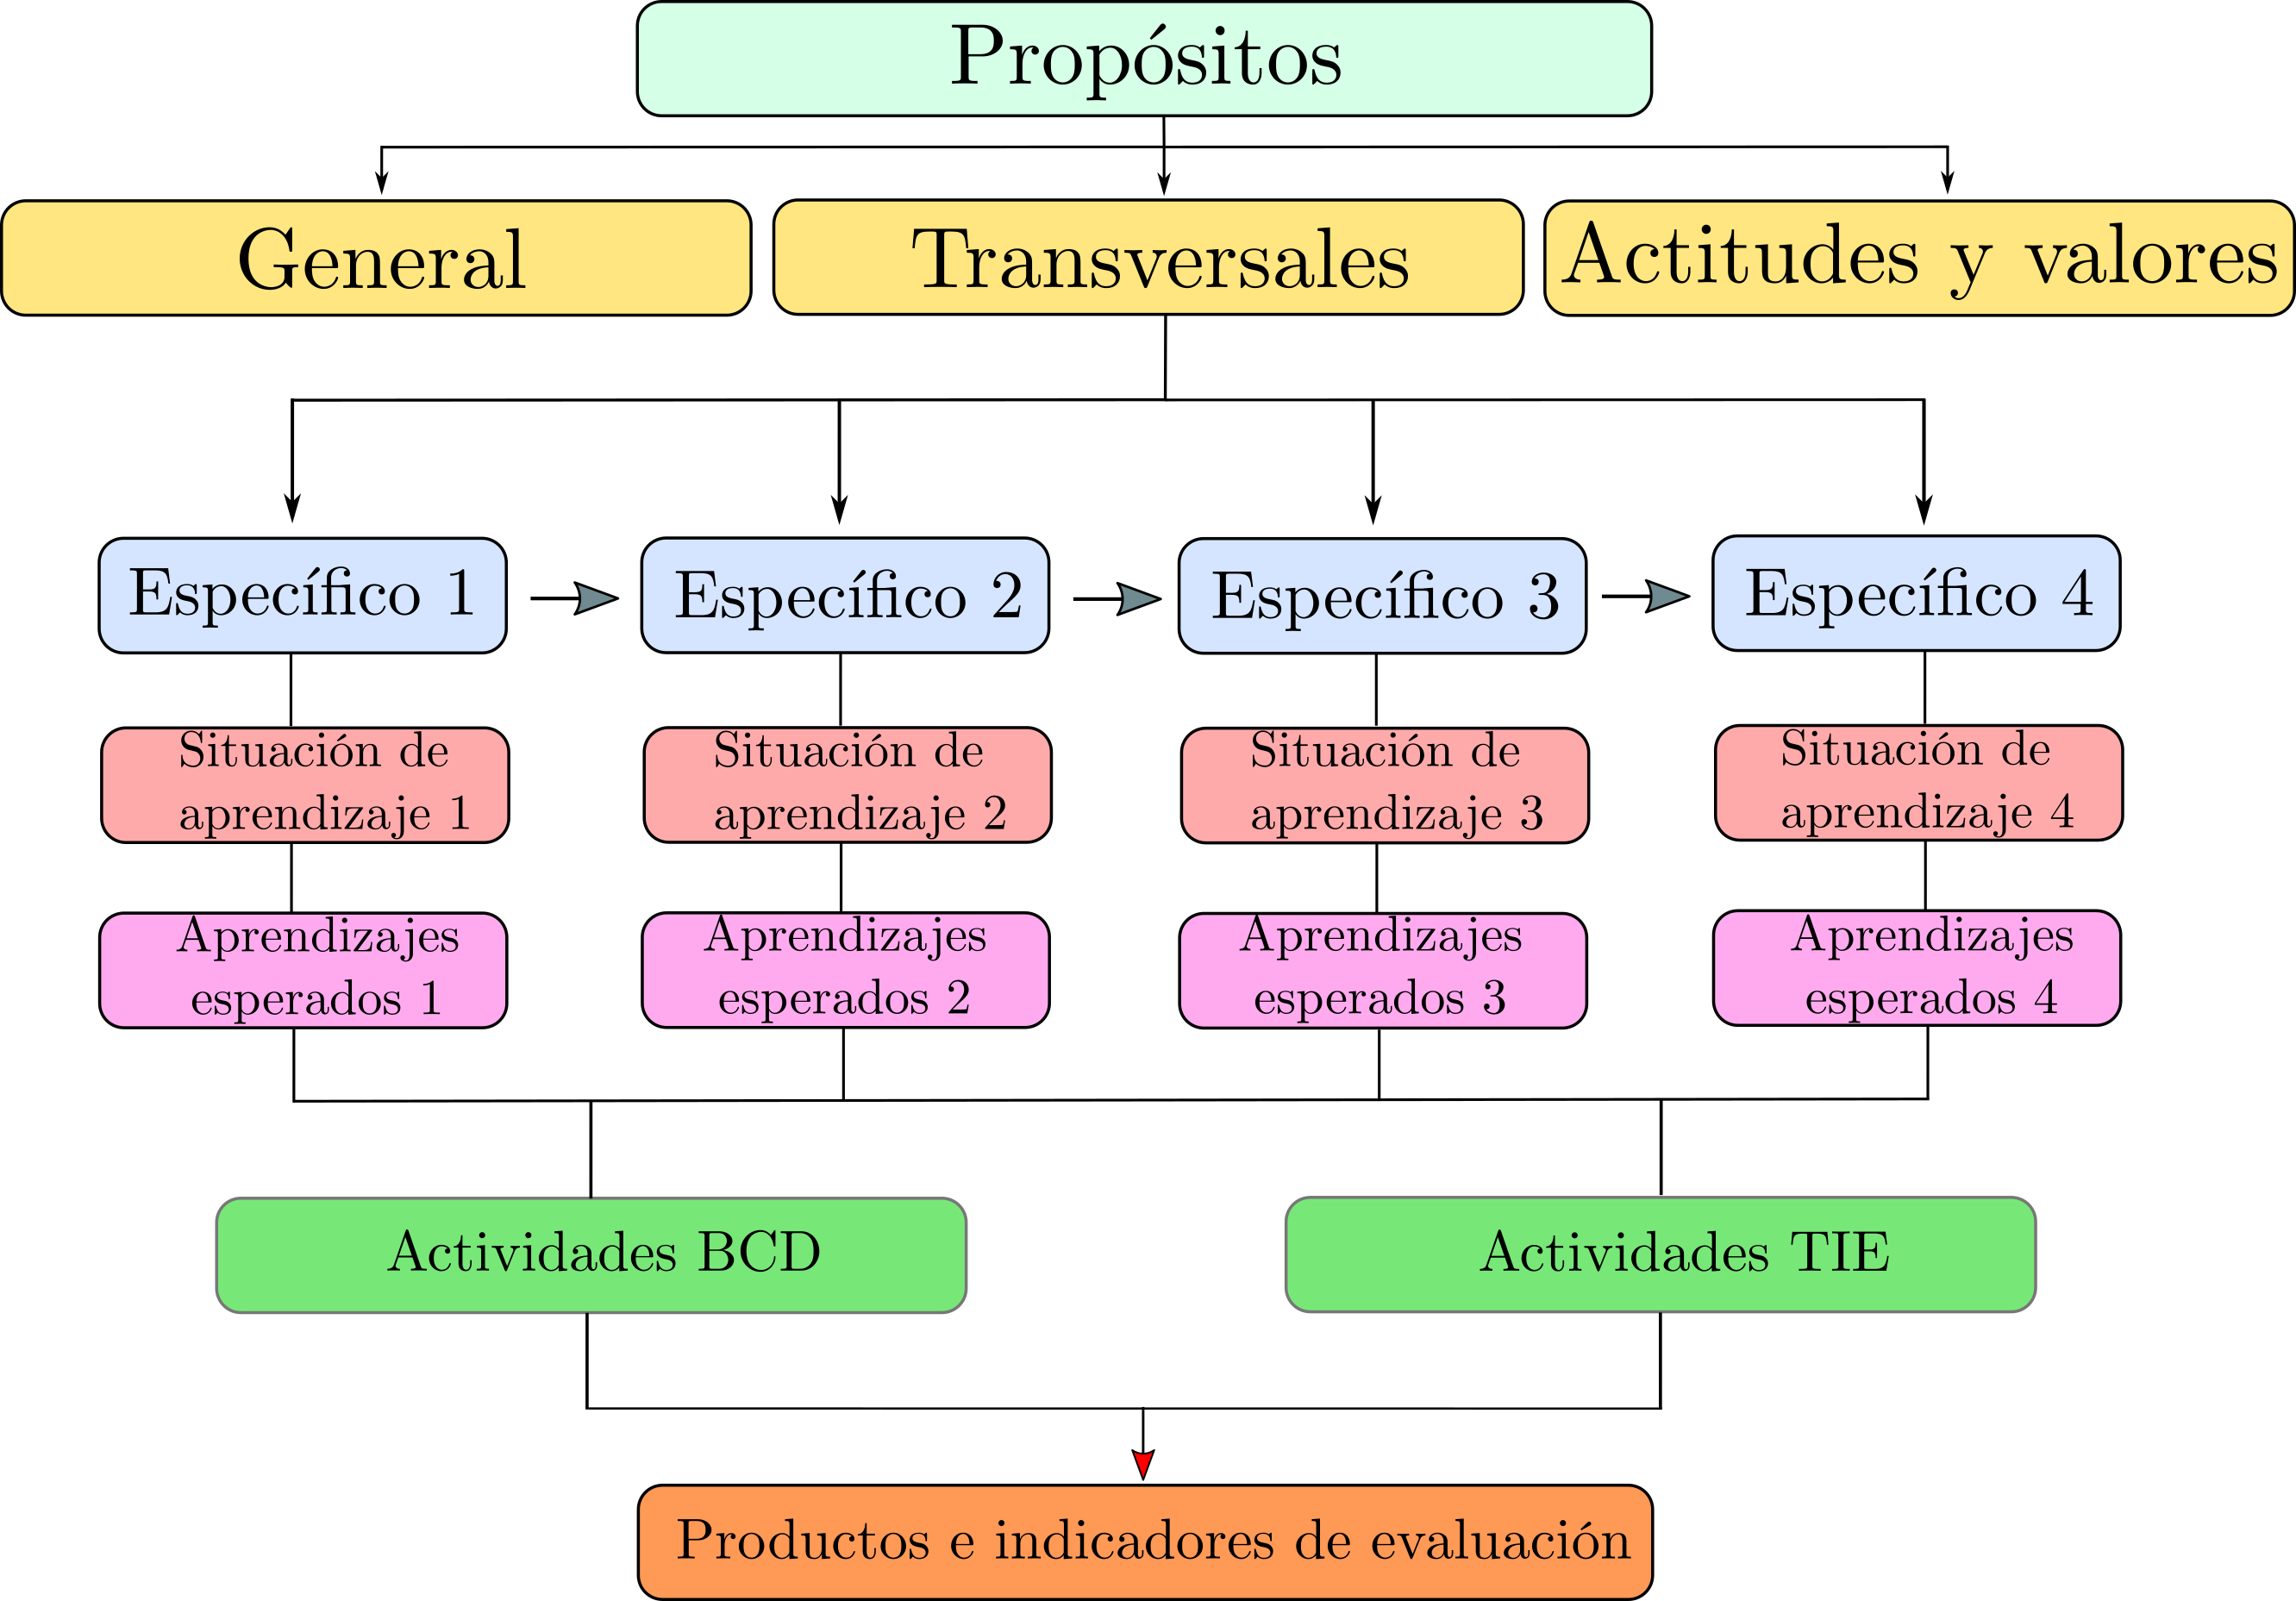
\includegraphics[scale=0.84]{mapa_iteso_gt}
	\end{figure}

\section{Propósitos}

\subsection{Propósito general}

Proporcionar al estudiante bases sólidas, como herramientas matemáticas y pensamiento estratégico, para modelar y resolver problemas de decisión en donde participa más de un agente racional (sean individuos o empresas), con una visión heurística en donde las decisiones de uno dependen de las acciones de otros agentes, a través de un método de formalización matemática y resolución de casos específicos


\subsection{Propósitos transversales}

\begin{tcolorbox}[colback=yelltcol!80]
	\begin{enumerate}[\thesubsection .1]
		\setlength{\itemsep}{0pt}
%		\setlength{\parskip}{0pt}
		\item Comprender la teoría básica de la teoría de juegos.
		\item Aplicar la teoría de juegos en problemas específicos de la economía, finanzas y en otros ejemplos que ilustren la importancia social de teoría de juegos.
		\item Realizar el proceso de la traducción que consiste en abstraer y modelar a partir de la descripción informal de una determinada situación a un problema formal de teoría de juegos.
		\item Reconocer aspectos y relaciones fundamentales en una situación financiera o administrativa.
		\item Transitar eficientemente entre representaciones matemáticas gráficas, verbales, tabulares y analíticas.
		\item Expresar de forma coherente y argumentada las estrategias utilizadas en la solución de problemas.
		\item Interpretar las soluciones obtenidas en el contexto de cada problema.
		\item Emplear software en la elaboración y operación de representaciones matemáticas en forma numérica, gráfica y analítica.
	\end{enumerate}
\end{tcolorbox}

\section{Actitudes y valores}

Se espera que al cursar esta asignatura desarrolles responsabilidad ante la actividad académica, manifiesta en al menos los siguientes aspectos:

\begin{itemize}
	\renewcommand\labelitemi{\faCheckCircle}
%	\setlength{\itemsep}{0pt}
%	\setlength{\parskip}{0pt}
	\item Participación activa, con compromiso, perseverancia y actitud positiva. 
	\item El cumplimiento de las normas de disciplina establecidas.
	\item El cumplimiento en tiempo y forma de las actividades que se te encomienden como trabajo independiente. 
	\item El desarrollo de espíritu crítico y autocrítico (constructivo) en el análisis del desempeño tuyo y de tus compañeros. 
	\item El sentido de la ética, evitando, en particular, cometer actos deshonestos en la realización de las actividades evaluativas.
	\item El desarrollo de la capacidad para identificar características personales al afrontar procesos de aprendizaje y, como consecuencia, para aprender con mayor independencia.
	\item Diálogo abierto, directo y respetuoso tanto con el profesor como con tus compañeros. 
	\item Tolerancia y respeto. 
\end{itemize}

\section{Propósitos específicos}

\begin{tcolorbox}[colback=bluerow!60]
	\subsection{Específico 1: }
		\begin{tight_enumerate}
			\item Presentación.
			\item Teoría de utilidad esperada (Tadelis, 2013;\textbf{ capítulos 1-3}).
			\item Juegos con Información completa y decisiones simultáneas (Tadelis, 2013;\textbf{ capítulos 3-6}).
		\end{tight_enumerate}
	\begin{mybox}[colback=redrow!80]{Situación de aprendizaje 1}
		 \textbf{Competencia de Cournot}: se resuelve el problema de competencia de producción de dos empresas líderes en el mercado, se generaliza a $n$ empresas y se explican brevemente las consecuencias de la competencia perfecta cuando $ n \rightarrow \infty $.
	\end{mybox}

	\begin{mybox}[colback=purplerow!80]{Aprendizajes esperados 1}
		\begin{tight_enumerate}
			\item Funciones de utilidad y decisiones bajo incertidumbre.
			\item La forma normal de un juego con estrategias puras. 
			\item Representación matricial: un juego finito de dos jugadores. 
			\item Dominancia en estrategias puras. 
			\item Eliminación iterativa de estrategias estrictamente dominadas. 
			\item El equilibrio de Nash en estrategias puras. 
			\item El equilibrio de Nash: algunas aplicaciones clásicas. 
			\item Estrategias, creencias y pagos esperados.
		\end{tight_enumerate}
	\end{mybox}
\end{tcolorbox}

% Propósito específico 2
\vspace*{1em}

\begin{tcolorbox}[colback=bluerow!60]
	\subsection{Específico 2: }
		Juegos con información completa y decisiones sucesivas (Tadelis, 2013; \textbf{capítulos 7-11}).
	\begin{mybox}[colback=redrow!80]{Situación de aprendizaje 2}
		\textbf{a)	Pánico bancario:} se modela una situación en la que dos agentes realizan una cierta inversión bancaria y deben decidir si retirar sus fundos antes o después de que la inversión llegue a su vencimiento.\\
		\textbf{b)	Henry Ford y el salario de 5 dólares:} se modela una situación en la que dos agentes tienen múltiples encuentros en la misma situación estratégica (juego de etapa simple), en donde un patrón decide el salario de sus trabajadores, y los trabajadores deciden si ser diligentes o no. Se enfatiza la importancia de este tipo de juegos dada su relación con el aprendizaje por refuerzo.
		
	\end{mybox}
	
	\begin{mybox}[colback=purplerow!80]{Aprendizajes esperados 2}
		\begin{tight_enumerate}
			\item Forma extensiva vs forma estratégica. 
			\item Descripción matemática de un árbol de decisión.
			\item Información perfecta vs información imperfecta con información completa.
			\item La representación en forma normal de juegos representados en forma extensiva. 
			\item Racionalidad secuencial e inducción hacia atrás. 
			\item Perfección en subjuegos. 
			\item Juegos repetidos en dos etapas. 
			\item Juegos repetidos infinitamente. 
			\item Negociación secuencial.
		\end{tight_enumerate}
	\end{mybox}
\end{tcolorbox}


\begin{tcolorbox}[colback=bluerow!60]
	\subsection{Específico 3: }
	Juegos bayesianos con al menos uno de los jugadores con información incompleta, en donde el jugador representa la incertidumbre mediante distribuciones de probabilidad (Tadelis, 2013); \textbf{capítulos 12-14}).
	\begin{mybox}[colback=redrow!80]{Situación de aprendizaje 3}
		\textbf{Subasta a sobre cerrado:} se modela una situación de subasta en la que las valoraciones de los participantes son información privada. Se comienza con dos jugadores y se generaliza rápidamente a $n$ jugadores.
	\end{mybox}
	
	\begin{mybox}[colback=purplerow!80]{Aprendizajes esperados 3}
		\begin{tight_enumerate}
			\item Representación estratégica de los juegos bayesianos. 
			\item Equilibrio bayesiano de Nash. 
			\item Revisión de las estrategias mixtas. 
			\item Subasta de sobre cerrado al primer precio y al doble precio. 
			\item El principio de revelación. 
			\item Lucha por el mercado con información asimétrica. 
			\item Estrategias dominantes y el mecanismo de designación de Vickrey-Clarke-Groves
		\end{tight_enumerate}
	\end{mybox}
\end{tcolorbox}

\vspace{1em}

\begin{tcolorbox}[colback=bluerow!60]
	\subsection{Específico 4: }
	Juegos bayesianos secuenciales con al menos uno de los jugadores con información incompleta, pero capaz de asignarles probabilidades (Tadelis, 2013; \textbf{capítulos 15-18}).
	\begin{mybox}[colback=redrow!80]{Situación de aprendizaje 4}
		Se modela un juego de señalización en el que no existe costo del mensaje como el anunció de política monetaria por parte de la autoridad monetaria.
	\end{mybox}
	
	\begin{mybox}[colback=purplerow!80]{Aprendizajes esperados 4}
		\begin{tight_enumerate}
			\item Introducción al equilibrio bayesiano perfecto.
			\item Equilibrio bayesiano perfecto en juegos de señalización.
			\item Inversión empresarial y estructura de capital.
			\item Juegos con parloteo (cheap-talk games).
			\item Política monetaria.
			\item Negociación sucesiva bajo información asimétrica.
			\item Refinamientos del equilibrio bayesiano perfecto.
		\end{tight_enumerate}
	\end{mybox}
\end{tcolorbox}

\section{Actividades bajo control docente y trabajo independiente del estudiante}

\noindent\begin{mybox}[width=.49\textwidth, nobeforeafter, colback=gray!10]{BCD}
	
\begin{tight_enumerate}
	\item Resolver problemas para construir y consolidar conocimiento.
	\item Resolver ejercicios operatorios.
	\item Definir y analizar conceptos y propiedades.
	\item Elaborar bosquejos y gráficas (con o sin software) de problemas de Teoría de Juegos.
	\item Usar software para resolver problemas que pueden ser modelados mediante la Teoría de Juegos.
	\item Colaborar con compañeros de equipo en la solución de problemas.
	\item Resolver exámenes.
	\item Elaborar un proyecto
\end{tight_enumerate}
	

\end{mybox}\hfill
\noindent\begin{mybox}[width=.49\textwidth, nobeforeafter, colback=gray!10]{TIE}
\begin{tight_enumerate}
	\item Resolver ejercicios y problemas para consolidar conocimiento.
	\item Investigar conceptos y propiedades.
	\item Elaborar bosquejos y gráficas (con o sin software) de problemas de Teoría de Juegos.
	\item Usar software para resolver problemas que pueden ser modelados mediante la Teoría de Juegos.
	\item Elaborar un proyecto final.
	\vspace{5em}
\end{tight_enumerate}
\end{mybox}

\section{Evaluación}

\begin{tcolorbox}
	\textbf{Productos esperados:}
	Ejercicios y problemas resuelto (Hojas de trabajo)
	
	\begin{mybox}{Indicadores de Evaluación}
		\textbf{En general:}
		\begin{itemize}
			\setlength{\itemsep}{0pt}
			\setlength{\parskip}{0pt}
			\item Entrega en tiempo y forma.
			\item Entrega de actividad completa.
			\item Limpieza y orden.
		\end{itemize}
		\textbf{En la solución de los problemas:}
		\begin{itemize}
			\setlength{\itemsep}{0pt}
			\setlength{\parskip}{0pt}
			\item Uso de estrategia adecuada al problema
			\item Desarrollo de procedimientos claros, completos y correctos.
			\item Uso correcto de la notación matemática.
			\item Reporte de resultados en las unidades correspondientes.
		\end{itemize}
		\textbf{En la interpretación de resultados:}
		\begin{itemize}
			\setlength{\itemsep}{0pt}
			\setlength{\parskip}{0pt}
			\item Claridad en la redacción y correcta ortografía.
			\item Redacción de respuesta en términos de la pregunta.
			\item Argumentación en base a los resultados numéricos y el contexto del problema.
		\end{itemize}
		
		En el caso de que se haya acordado que podía utilizarse software debe presentarse la evidencia el uso del correcto la notación del programa y los resultados obtenidos.
		
	\end{mybox}
\end{tcolorbox}

\begin{tcolorbox}
	\textbf{Productos esperados:}
	Cuestionarios sobre conceptos y propiedades
	
	\begin{mybox}{Indicadores de Evaluación}
		\textbf{En general:}
		\begin{itemize}
			\setlength{\itemsep}{0pt}
			\setlength{\parskip}{0pt}
			\item Entrega en tiempo y forma.
			\item Entrega de actividad completa.
			\item Limpieza y orden.
			
		\end{itemize}
		\textbf{En la respuesta:}
		\begin{itemize}
			\setlength{\itemsep}{0pt}
			\setlength{\parskip}{0pt}
			\item Desarrollo completo, correcto y en términos de la pregunta.
			\item Uso correcto de la notación matemática.
			\item Claridad en la redacción y correcta ortografía.
		\end{itemize}
	\end{mybox}

	\textbf{Productos esperados:}
	Bosquejos y gráficas (Hojas de trabajo/Reportes de práctica)
	
	\begin{mybox}{Indicadores de Evaluación}
		\textbf{En general:}
		\begin{itemize}
			\setlength{\itemsep}{0pt}
			\setlength{\parskip}{0pt}
			\item Entrega en tiempo y forma.
			\item Entrega de actividad completa.
			\item Limpieza y orden.			
		\end{itemize}
		\textbf{En los bosquejos o gráficas:}
		\begin{itemize}
			\setlength{\itemsep}{0pt}
			\setlength{\parskip}{0pt}
			\item Uso del método acordado (manual o software).
			\item Asignación, etiquetado y escala adecuada en los ejes.
			\item Identificación de puntos o zonas mediante notación de puntos o intervalos.
		\end{itemize}
	\end{mybox}

	\textbf{Productos esperados:}
	Exámenes
	\begin{mybox}{Indicadores de Evaluación}
		\textbf{En general:}
		\begin{itemize}
			\setlength{\itemsep}{0pt}
			\setlength{\parskip}{0pt}
			\item Entrega en tiempo y forma.
			\item Entrega de actividad completa.
			\item Limpieza y orden.			
		\end{itemize}
		\textbf{En la solución de los problemas:}
		\begin{itemize}
			\setlength{\itemsep}{0pt}
			\setlength{\parskip}{0pt}
			\item Uso de estrategia adecuada al problema
			\item Desarrollo de procedimientos claros, completos, correctos y uso de la notación matemática.
			\item Reporte de resultados en las unidades correspondientes.	
		\end{itemize}
		\textbf{En la interpretación de resultados:}
		\begin{itemize}
			\setlength{\itemsep}{0pt}
			\setlength{\parskip}{0pt}
			\item Claridad en la redacción y correcta ortografía.
			\item Redacción de respuesta en términos de la pregunta.
			\item Argumentación en base a los resultados numéricos y el contexto del problema.
		\end{itemize}
		\textbf{En los bosquejos o gráficas:}
		\begin{itemize}
			\setlength{\itemsep}{0pt}
			\setlength{\parskip}{0pt}
			\item Asignación, etiquetado y escala adecuada en los ejes.
			\item Identificación de curvas y superficies graficados.
			\item Identificación de puntos o zonas mediante notación de puntos o intervalos.
		\end{itemize}
	\end{mybox}

\end{tcolorbox}

\begin{tcolorbox}
	\textbf{Productos esperados:}
	Proyectos
	
	\begin{mybox}{Indicadores de Evaluación}
		\textbf{En general:}
		\begin{itemize}
			\setlength{\itemsep}{0pt}
			\setlength{\parskip}{0pt}
			\item Entrega en tiempo y forma.
			\item Entrega de actividad completa.
		\end{itemize}
		\textbf{En la información:}
		\begin{itemize}
			\setlength{\itemsep}{0pt}
			\setlength{\parskip}{0pt}
			\item Selección de tema relacionado con las carreras de los integrantes.
			\item Selección adecuada de datos
			\item Autentificación datos.
		\end{itemize}
		\textbf{En el reporte:}
		\begin{itemize}
			\setlength{\itemsep}{0pt}
			\setlength{\parskip}{0pt}
			\item Limpieza y orden.
			\item Claridad en la redacción y correcta ortografía.
			\item Desarrollo completo y correcto de los apartados requeridos en el proyecto.
			\item Elaboración del reporte escrito, de las gráficas y las tablas con los programas convenidos.
		\end{itemize}
		\textbf{En los cálculos:}
		\begin{itemize}
			\setlength{\itemsep}{0pt}
			\setlength{\parskip}{0pt}
			\item Uso correcto de la notación matemática.
			\item Respaldo de cada paso en definiciones, propiedades y teoremas.
		\end{itemize}
		\textbf{En la colaboración:}
		\begin{itemize}
			\setlength{\itemsep}{0pt}
			\setlength{\parskip}{0pt}
			\item Selección voluntaria de integrantes; tres integrantes.
			\item Reparto equitativo de actividades.
			\item Desempeño de integrantes según lo acordado.
		\end{itemize}
		\textbf{Bibliografía}
		\begin{itemize}
			\setlength{\itemsep}{0pt}
			\setlength{\parskip}{0pt}
			\item Uso del tipo de fuentes acordadas.
			\item Hacer citas con formato APA.
		\end{itemize}
	\end{mybox}
\end{tcolorbox}

\textbf{Evaluación del aprendizaje}

\begin{table}[ht]
	\centering
	\begin{tabular}{|l|l|}
		\hline
		\rowcolor[HTML]{D9D9D9} 
		Productos     & \% de Calificación \\ \hline
		Exámenes (4)  & 60 \% \\ \hline
		Tareas        & 40\%  \\ \hline
		&                                                                 \\
		TOTAL:        & 100\\
		\hline                              
	\end{tabular}
\end{table}

\textbf{Contenido de exámenes}

\begin{table}[ht]
\centering
\begin{tabular}{|l|l|}
	\hline
	Primer examen parcial & Juegos estáticos de información completa.   \\ \hline
	Segundo examen        & Juegos dinámicos de información completa.  \\ \hline
	Tercer examen parcial & Juegos estáticos de información incompleta. \\ \hline
	Cuarto examen parcial & Juegos dinámicos de información incompleta. \\ \hline           
\end{tabular}
\end{table}

%\section{Información adicional}
%
%Se estará usando el lenguaje/entorno de programación {\sf\color{blue} \textbf{R}} con IDE {\sf\color{blue} \textbf{RStudio}}. Ambos son proyectos gratuitos, disponibles para todas las plataformas (Windows, macOS y Linux) en las siguientes ligas:
%
%\begin{itemize}
%	\item {\sf\color{blue} \textbf{R}}: \url{https://cran.r-project.org/}
%	\item {\sf\color{blue} \textbf{RStudio}}: \url{https://rstudio.com/products/rstudio/download/}
%\end{itemize}
%
% Deberán instalarse las siguientes librerías: {\color{blue} \texttt{lpSolve, lpSolveAPI, Rglpk}}.

\section{Bibliografía primaria y sugerida}

\subsection{Primaria:}

\begin{itemize}
	\item Tadelis, S. (2013). \textit{Game theory: an introduction.} Princeton University Press.
%	\item Sallan, J.M., Lordan, O. \& Fernandez, V. (2015). \textit{Modeling and solving Linear Programming with R.} OmniaScience. \\
%	Disponible gratuitamente en:\\ \url{https://www.omniascience.com/books/index.php/scholar/catalog/book/34}.
	\item Gibbons, R. 1992. \textit{Un primer curso de Teoría de Juegos}. Antoni Bosch.
\end{itemize}

\subsection{Sugerida:}

\begin{itemize}
	\item Harrington, Joseph.\textit{ Games, strategies and decision making}. Macmillan, 2009.
	\item Leyton-Brown, K., \& Shoham, Y. (2008). \textit{Essentials of game theory: A concise multidisciplinary introduction.} Synthesis lectures on artificial intelligence and machine learning, 2(1), 1-88.
	\item Thie, P. R., \& Keough, G. E. (2011). \textit{An introduction to linear programming and game theory.} John Wiley \& Sons.
	
\end{itemize}

\end{document}